\documentclass[times,t]{beamer}
\usepackage{amssymb}
\usepackage{amsmath}
\usepackage{amsfonts}
\usepackage{lmodern} 
\input{sym.tex}
\setbeamertemplate{navigation symbols}{}

\title{ECE 417/598: Direct Linear Transform }
\author{Vikas Dhiman}
\date{March 23, 2022}
\DeclareMathOperator{\diag}{diag}
\begin{document}

\newcommand{\ubfu}{\underline{\bfu}}
\newcommand{\ubfx}{\underline{\bfx}}
\begin{frame}
  \titlepage
  \end{frame}

\begin{frame}{Homography}
  \includegraphics[width=\linewidth]{media/homography-maps-a-line-to-a-line.png}
\end{frame}

\begin{frame}{Examples  of  Homography}
  \includegraphics[width=\linewidth]{media/examples-of-homography.png}
\end{frame}

\begin{frame}
  \includegraphics[width=0.60\linewidth]{media/audi top view camera.jpg}
\end{frame}

\begin{frame}{Computing Homography}
  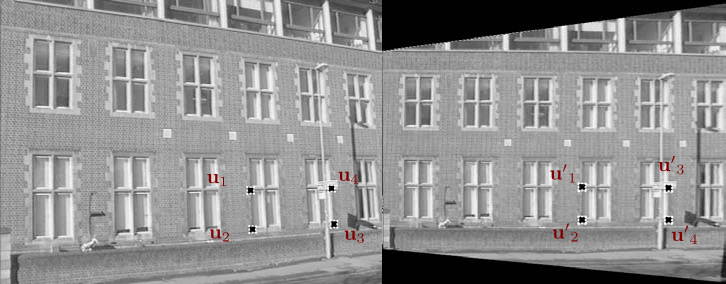
\includegraphics[width=\linewidth]{media/removing-perspective-distortion.png.pdf}
  \begin{align*}
    \ubfu_1 &= [100, 98, 1]^\top&
    \ubfu_2 &= [102, 95, 1]^\top\\
    \ubfu_3 &= [107, 90, 1]^\top&
    \ubfu_4 &= [110, 85, 1]^\top \\
    \ubfu'_1 &= [100, 98, 1]^\top&
    \ubfu'_2 &= [102, 95, 1]^\top\\
    \ubfu'_3 &= [107, 98, 1]^\top&
    \ubfu'_4 &= [110, 95, 1]^\top
  \end{align*}
  Find $H$ such that $\ubfu' = H\ubfu$ for any point on one image to another
  image, where $\ubfu', \ubfu \in \bbP^2$
\end{frame}

\begin{frame}{2D homography}
  Given a set of points $\ubfu_i \in \bbP^2$ and a corresponding set of
  points $\ubfu'_i \in \bbP^2$, compute the projective transformation that takes each
  $\ubfu_i$ to $\ubfu'_i$ . In a practical situation, the points $\ubfu_i$ and   $\ubfu'_i$  are points in two images
  (or the same image), each image being considered as a projective plane  $\bbP^2$.
\end{frame}

\begin{frame}{Solving for Homography }
\end{frame}

\begin{frame}{Solving for Homography }
\end{frame}

\begin{frame}{Solving for Homography }
  \includegraphics[width=\linewidth]{media/homography-code.png}
\end{frame}
\begin{frame}
  Apply Homography
  \includegraphics[width=\linewidth]{media/apply-homography-code.png}
\end{frame}

\begin{frame}{3D  to  2D camera projection matrix estimation}
  Given a set of points $\bfX_i$ in 3D space, and a set
  of corresponding points $\bfx_i$ in an image, find the 3D to 2D projective
  $\bfP$ mapping
  that maps $\bfX_i$ to $\bfx_i  =  \bfP\bfX_i$.
\end{frame}

\end{document}